\chapter{導入}

この集中講義ではPCP定理と呼ばれる計算量理論の基本的な結果について解説し, その証明を与える.
PCP定理は1998年に\citet{AroraS98,AroraLMSS98}によって証明された.
この証明は代数的な手法に基づく誤り訂正符号を技巧的に組合せたものであり, 難解なものであったが, その後\citet{Din07}によってより簡潔な証明が与えられた.
この講義では\citet{Din07}による比較的簡単な証明を紹介する.
ちなみにDinurはのちにこの業績によりゲーデル賞を受賞している.

\section{計算量理論の復習}
まずは計算量理論のどの教科書にも載っているような基礎的な用語の定義を与える.
なお, このノートではアルゴリズムの定義 (チューリング機械の定義) は省略し, アルゴリズムについて述べる際は具体的な計算の手続きを述べる\footnote{ひとまずPythonやC言語などで実装されたプログラムを考えれば良い. ただし, 計算機内では全ての数値は有限桁の二進数で表記されており, その読み書きや演算には少なくとも桁数に比例した計算時間がかかる. なお, $\sqrt{2}$といった無理数は本来は有限桁で打ち切った近似値を扱うが, そのような小数はこの講義では扱わず, 特に断りのない限りは整数値のみを考える. また, 記憶領域へのアクセスは定数時間で行えると仮定する(チューリング機械であればテープの移動にかかる時間も考慮する).}.

まずは基本的な記号の定義を与える:
\begin{itemize}
\item オーダー記法: 二つの関数$f,g\colon\Nat\to\Nat$に対し, $f(n)=O(g(n))$であるとは, ある定数$c>0$が存在して, 十分大きな全ての$n\in\Nat$に対して$f(n)\le cg(n)$が成り立つことをいう. また, $f(n)=\Omega(g(n)), f(n)=o(g(n)), f(n)=\omega(g(n))$なども同様に($n\to\infty$として)定義する.
\item 自然数$n\in\Nat$に対して$[n]=\qty{1,\dots,n}$とする.
\item $\binset^*=\bigcup_{n\in\Nat}\binset^n$を有限長の二進文字列全体とする.
\item $x\in\binset^*$に対して$\abs{x}$を$x$の文字数とする.
\item アルゴリズム$A$に対し, $A(x)$を入力$x \in \binset^*$に対するアルゴリズム$A$の出力とする. ここで, 単に「アルゴリズム」と言った場合は決定的アルゴリズムを指し, 乱択アルゴリズムについては明示的に言及する.
\item 関数$T(n)\colon\Nat\to\Nat$を考える. 十分大きな全ての$n\in\Nat$と全ての$x\in\binset^n$に対して, $A$が$A(x)$を出力するまでにかかる計算ステップ数の最大値が高々$T(n)$であるとき, アルゴリズム$A$の計算量は$T(n)$であるという. 特に, ある($n$に依らない)定数$c>0$が存在して計算量が$O(n^c)$で抑えられるアルゴリズムを\emph{多項式時間アルゴリズム}という\footnote{計算モデルによって一つ一つの計算ステップの定義は異なるが, 原理的には1bitの演算や記憶領域への読み書きの回数と思えばよい. 多項式時間で動くかどうかの議論であれば, 多くの古典的な計算モデルは等価である.}
\item 慣例的な記法だが, 二つの文字列$x,y\in\binset^*$を入力として受け取るアルゴリズムは$A(x,y)$と表す. 三つ以上の場合も$A(x,y,z)$などと表す.
\end{itemize}

計算量理論で最も基本的な問題群として判定問題と呼ばれる問題群がある.

\begin{definition}{判定問題}{decision-problem}
  部分集合$L\subseteq\binset^*$を\emph{判定問題(または言語)}という.
  また, 文字列$x\in\binset^*$は$x\in L$であるとき, 判定問題$L$の\emph{Yesインスタンス}といい,
  そうでない場合は\emph{Noインスタンス}という.

  文字列$x\in\binset^*$に対し$L(x)\in\binset$を, $x\in L$かどうかの指示関数, すなわち$x\in L$ならば$L(x)=1$, そうでなければ$L(x)=0$と定義する.

  アルゴリズム$A$は, 任意の$x\in\binset^*$に対して$A(x)=L(x)$が成り立つとき,
  $A$は$L$を解くという.
\end{definition}

この講義では「効率的に解ける」といった場合, 多項式時間アルゴリズムによって解けることを指す. そのような判定問題の集合をクラスPという.
\begin{definition}{クラスP}{classP}
  判定問題$L$は, それを解く多項式時間アルゴリズムが存在するとき, $\P$に属するという.
\end{definition}

次に乱択アルゴリズムについて定義する. 端的に言えばアルゴリズムの内部でコイントスを行うものを乱択アルゴリズムという.
ここでは明示的にランダムシードを受け取るアルゴリズムを乱択アルゴリズムと呼ぶことにする.

\begin{definition}{乱択アルゴリズム}{randomized-algorithm}
  入力$x\in\binset^*$とは別にランダムシード(乱数表)と呼ばれる別の文字列$s\in\binset^*$を受け取るアルゴリズムを\emph{乱択アルゴリズム}といい, ランダムシードであることを強調するために$A(x;s)$などと表す.
  なお, 任意の$x,s\in\binset^*$に対して$A(x;s)$は有限時間で停止するとし, その計算量は$\abs{x}$のみに依存する関数で表せるとする.
  このとき, ランダムシード$s$の長さを常に$A$の計算量で上から抑える.
  すなわち, $A$の計算量が$T(n)$であるとき, 十分大きな全ての$n\in\Nat$と全ての$x\in\binset^n$に対して$A$が読み込む$s$の文字数は高々$T(n)$であるため, $s\in \binset^{T(n)}$であると仮定する.
  しばし, ランダムシード$s$を明記する必要が特にない場合は$A(x)$と表す.

  乱択アルゴリズムのランダムシードに関する確率, 期待値, 分散を議論する際は記号として$\Pr_{A}[\cdot],\E_A[\cdot],\Var_A[\cdot]$を用いる.
  乱択アルゴリズム$A$が判定問題$L$を解くとは,
  \begin{align*}
    \Pr_A[A(x)=L(x)]\geq 2/3
  \end{align*}
  が成り立つことをいう.
\end{definition}

また, 入力とは別に文字列へのオラクルアクセスを受け取るアルゴリズムを考える.
\begin{definition}{オラクルアルゴリズム}{oracle-algorithm}
  文字列$\pi\in\binset^*$に対し, $\pi$への\emph{オラクルアクセス}を持つアルゴリズム$A^\pi(x)$とは, 計算途中で$\pi$の指定された位置の文字を読むことができるアルゴリズムである.
  すなわち, $\pi$の$i$番目の文字を読む操作を$A^\pi(x)$の計算過程中に$O(\log \abs{\pi})$時間で行うことができるアルゴリズムである.\footnote{自然数$i\in[\abs{\pi}]$を指定するために$O(\log \abs{\pi})$ビットを定めなければならないため, $O(\log \abs{\pi})$時間を仮定している.}
  同様に乱択オラクルアルゴリズムについても定義できる.
\end{definition}


\section{検証の計算量}
数学全般における検証とは, ある命題が真であると主張する証明が与えられたとき, その証明が実際に
その命題を正しく証明しているかどうかを確認することを意味する.
論文や記述試験の証明の査読や採点をイメージしてもらうとわかりやすいだろう.
計算量理論では検証やその計算量の議論は重要な研究テーマであり, その検証に要する計算量が議論される.

\subsection{効率的な検証とクラスNP}
判定問題$L$と入力$x\in\binset^*$を与えられたとき, $x\in L$かどうかを審議したい.
ここで$x\in L$を主張する証明が文字列$\pi\in\binset^*$で与えられたとする.
このとき, \emph{検証者}と呼ばれるアルゴリズムは$x$と$\pi$を読み込んで$x\in L$かどうかを判定する.
この判定を多項式時間で行えるとき, その判定問題$L$の集合を$\NP$という.

\begin{definition}{クラスNP}{classNP}
  判定問題$L$は, 以下を満たす多項式時間アルゴリズム$V$と多項式$p\colon\Nat\to\Nat$が存在するとき, $L$は$\NP$に属するという:
  アルゴリズム$V$は入力として$x,\pi\in\binset^*$を受け取り, $0$または$1$を出力する.
  \begin{enumerate}
  \item もし$x\in L$ならば, ある$\pi\in\binset^{p(\abs{x})}$が存在して$V(x,\pi)=1$となる.
  \item もし$x\notin L$ならば, 全ての$\pi\in\binset^{p(\abs{x})}$に対して$V(x,\pi)=0$となる.
  \end{enumerate}
  また, このようなアルゴリズム$V$を\emph{NP検証者}といい, $\pi$を\emph{NP証拠}という.
\end{definition}

\begin{remark}{クラスPとNPの関係}{remark.P-NP}
  判定問題$L$が$\P$に属するならば$L\in\NP$である.
  実際, 受け取った$x\in\binset^*$に対して$L(x)$を計算してそれを出力する検証者を考えばよい.
  すなわち$\P\subseteq\NP$である.
  一方, 逆側の包含関係$\NP\subseteq\P$が成り立つかどうかはP vs NP問題と呼ばれる計算量理論における最も重要な未解決問題であり, 多くの研究者は$\NP\subseteq\P$が成り立たないと信じている.
\end{remark}

\begin{example}{合成数判定問題}{ex.composite-number-problem}
  判定問題$L=\{x\in\binset^*\colon x\text{は合成数}\}$を考える.
  このとき, 検証者は$x$と$\pi$を読み込んで, $\pi\not\in\{1,x\}$かつ$\pi$が$x$を割り切るかどうかを判定する.
  もしも$x\in L$である場合, 合成数なので非自明な約数を証拠$\pi$として与えれば$V(x,\pi)=1$となる.
  そうでない場合, 非自明な約数は存在しないため必ず$V(x,\pi)=0$となる.
  このアルゴリズム$V$は入力長(つまり数値の二進表現したときのビット長)に関する多項式時間で動作するため, $L$はNPに属する.
\end{example}

\begin{example}{グラフ彩色問題}{ex.graph-coloring-problem}
  自然数$k\ge 2$とグラフ$G=(V,E)$に対し, 関数$c\colon V\to[k]$が
  全ての辺$\{u,v\}\in E$に対して$c(u)\neq c(v)$を満たすとき, $c$を$G$の$k$-彩色といい,
  $k$-彩色が存在するようなグラフは$k$-彩色可能であるという.
  任意の$k\ge 2$に対し, 判定問題
  $$L=\{G\in\binset^*\colon G\text{は}k\text{-彩色可能}\}$$
  はNPに属する.
  検証者は$G$と$\pi$を読み込んで, $\pi$が$G$の$k$-彩色であるかどうかを判定する.
  もしも$G\in L$である場合, $G$は$k$-彩色可能であるため, $k$-彩色の証拠$\pi$を与えれば$V(G,\pi)=1$となる.
  そうでない場合, $G$は$k$-彩色可能でないため必ず$V(G,\pi)=0$となる.
  このアルゴリズム$V$は多項式時間で動作するため, $L$はNPに属する.
\end{example}

\begin{exercise}{素数判定問題}{exer.prime-problem}
  自然数$n\in\Nat$に対し, 判定問題$\PRIMES=\{a\in\Nat\colon a\text{は素数}\}$を考える.
  この問題は$\P$に属することが知られている\cite{AKS04}が, その複雑なアルゴリズムを用いずに
  初等的に$\PRIMES\in \NP$を示したい.
  そのために, 以下の事実を用いる:

  任意の自然数 $a\in\Nat$と$\gamma\in\{1,\dots,a-1\}$に対し, $\gamma^0,\gamma^1,\dots \pmod a$は周期的である. さらに, 以下が成り立つ:
  \begin{itemize}
  \item $a$が素数であるならば, ある$\gamma\in\{1,\dots,a-1\}$が存在して$\gamma^0,\gamma^1,\dots \pmod a$の周期が$a-1$である\footnote{このような$\gamma$を原始元という.}.
  \item 一方, $a$が素数でないならば, 全ての$\gamma\in\{1,\dots,a-1\}$に対して$\gamma^0,\gamma^1,\dots \pmod a$の周期は$a-1$未満である. 特に, その周期$L$は$a-1$を割り切る.
  \end{itemize}
  これらの事実を用いて, 以下の小問に答えよ.

  \begin{enumerate}
  \item 次の検証者$V_1$を考える: 入力$a\in\Nat$と証拠$\gamma\in\{1,\dots,a-1\}$に対し, $\gamma^0,\gamma^1,\dots,\gamma^{a-2} \pmod a$を全て検証し, これら全て相異なるかどうかを判定する. この検証者$V_1$が多項式時間アルゴリズム\emph{でない}理由を簡潔に説明せよ.
  \item 入力$a\in\Nat$に対し, $a$が素数であることの証拠として, 原始元$\gamma\in\{1,\dots,a-1\}$および$a-1$の素因数分解$a-1=p_1^{\alpha_1}\cdots p_k^{\alpha_k}$および各$p_i$が素数であることの証拠を再帰的に与える. この証拠を用いて, 検証者$V_2$は$a$が素数であるかどうかを多項式時間で判定できることを示せ.
  \end{enumerate}
\end{exercise}

\subsection{局所的な検証とクラスPCP}

一般に$x\in L$かどうかの検証では, 証明$\pi$の全ての文字を読む必要がある.
しかし, 証明$\pi$のうちの一部の文字を読むだけで$x\in L$かどうかを\emph{確率的に}判定できる場合がある.
そのような性質を持つ証拠を\emph{確率的検証可能な証拠}(Probabilistically Checkable Proof, PCP)という.

\begin{figure}[htbp]
  \centering
  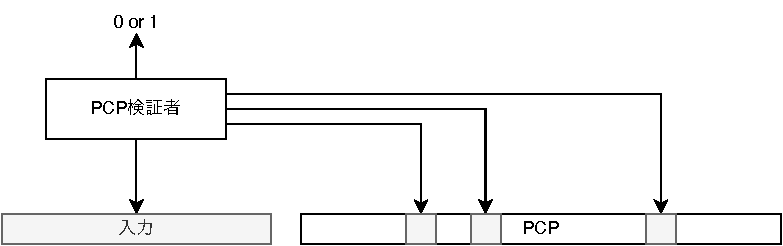
\includegraphics[width=0.8\textwidth]{images/PCPverifier.drawio.pdf}
  \caption{確率的検証可能な証拠の概念図. 検証者は乱数を用いて証拠$\pi$のうちの一部の文字のみを読み, それに基づいて判定を行う.}
  \label{fig:pcpverifier}
\end{figure}


\begin{definition}{確率的検証可能な証拠}{PCP}
  二つの関数$r,q\colon\Nat\to\Nat$に対し, $\PCP(r,q)$を以下の性質を持つ判定集合$L$の集合とする: ある多項式時間オラクル乱択アルゴリズム$V$が存在して, 任意の$x\in\binset^*$に対し,
  \begin{enumerate}
  \item もし$x\in L$ならば, ある$\pi\in\binset^*$が存在して, ($V$の乱択に関して)確率$1$で$V^\pi(x)=1$となる (\emph{完全性}).
  \item もし$x\notin L$ならば, 全ての$\pi\in\binset^*$に対して, ($V$の乱択に関して)確率$1/3$以上で$V^\pi(x)=0$となる (\emph{健全性}).
  \item さらに, 入力長が$n=\abs{x}$のとき, $V^\pi(x)$はオラクル$\pi$のうち高々$q(n)$個の文字を読み, そのランダムシード長は$r(n)$で抑えられる.
  \end{enumerate}
  このようなオラクル乱択アルゴリズム$V$を\emph{PCP検証者}といい, 証拠$\pi$を\emph{PCP}という.
\end{definition}
\begin{remark}{PCPの長さ}{PCP-length}
  $\PCP(r,q)$の証拠$\pi$の長さは$q(n)2^{r(n)}$で抑えられる.
  各ランダムシード$s \in \binset^{r(n)}$に対して検証者は$\pi$のうち高々$q(n)$個の文字を読むため, 全てのランダムシードを列挙すると, アクセスされる可能性のある$\pi$の文字数は高々$q(n)2^{r(n)}$で抑えられる.
\end{remark}

一般にランダムシード長$r(n)$と読み込む文字数$q(n)$が小さいほど良いPCP検証者であると考えられる.
PCP検証者の構成は非常に難しい.
例えば\cref{ex:ex.graph-coloring-problem}のグラフ彩色問題に対する次の検証者を考えてみよう:
入力としてグラフ$G=(V,E)$と証拠として関数$\pi\colon V\to[k]$を受け取り, この関数$\pi$が実際に$G$の$k$-彩色であるかどうかを判定する.
検証者は$G$の辺$\{u,v\}\in E$をランダムに一つ選び, $\pi(u)\neq \pi(v)$であるかどうかによって判定する.
この検証者は$\pi$のうち高々$q(n)=O(1)$個の文字を読み, そのランダムシード長は$r(n)=O(\log n)$で抑えられる.
しかし, この検証者は健全性の条件を満たさない.
実際, $G$が$k$-彩色可能でない場合, どのような関数$\pi\colon V \to [k]$を与えても, 少なくとも一つの辺$\{u,v\}\in E$が存在して$\pi(u)=\pi(v)$となるが, 検証者がこのような辺を引き当てる確率は最悪の場合, $1/\abs{E}$となるからである.

PCP定理とは, ある$r(n)=O(\log n)$, $q(n)=O(1)$に対して$\PCP(r,q)=\NP$が成り立つことを主張する定理である.
例えばグラフ彩色問題は$\NP$に属するため, 実は全段落の$r(n),q(n)$を達成するPCP検証者が存在するのである!

\begin{theorem}{PCP定理}{PCPtheorem}
  ある$r(n)=O(\log n)$, $q(n)=O(1)$に対して$\PCP(r,q)=\NP$が成り立つ.
\end{theorem}

\begin{remark}{片側の包含関係}{one-sided-inclusion}
  PCP定理において, $\PCP(r,q)\subseteq \NP$は容易に示すことができる.
  実際, \cref{rem:PCP-length}により, 証拠$\pi$の長さは$q(n)2^{r(n)} = n^{O(1)}$で抑えられる.
  また, $r(n)=O(\log n)$より, 検証者は$2^{r(n)}=n^{O(1)}$個のランダムシードを列挙し, それら全てに対してPCP検証者を適用し, その出力値の多数決をとることで, 入力$x$に対して$x\in L$かどうかを多項式時間で判定できる.
  PCP定理の証明の本質的な難しさは逆側の包含関係$\NP\subseteq \PCP(r,q)$の証明にある.
\end{remark}

\section{PCP定理の応用}
PCP定理の応用として, 様々な組合せ最適化問題に対する近似のNP困難性を導出することができる.
